% Created 2018-11-12 月 12:48
% Intended LaTeX compiler: pdflatex
\documentclass[dvipdfmx,11pt]{jarticle}
\usepackage[utf8]{inputenc}
\usepackage[T1]{fontenc}
\usepackage{graphicx}
\usepackage{grffile}
\usepackage{longtable}
\usepackage{wrapfig}
\usepackage{rotating}
\usepackage[normalem]{ulem}
\usepackage{amsmath}
\usepackage{textcomp}
\usepackage{amssymb}
\usepackage{capt-of}
\usepackage{hyperref}
\setlength{\textwidth}{20cm}
\setlength{\oddsidemargin}{-1cm}
\setlength{\evensidemargin}{-1cm}
\setlength{\topmargin}{-3cm}
\setlength{\textheight}{28cm}
\author{鈴木正幸,非常勤講師}
\date{\today}
\title{コンピュータと数式処理}
\begin{document}

\maketitle

\section{概要}
\label{sec:orge857d94}
\begin{center}
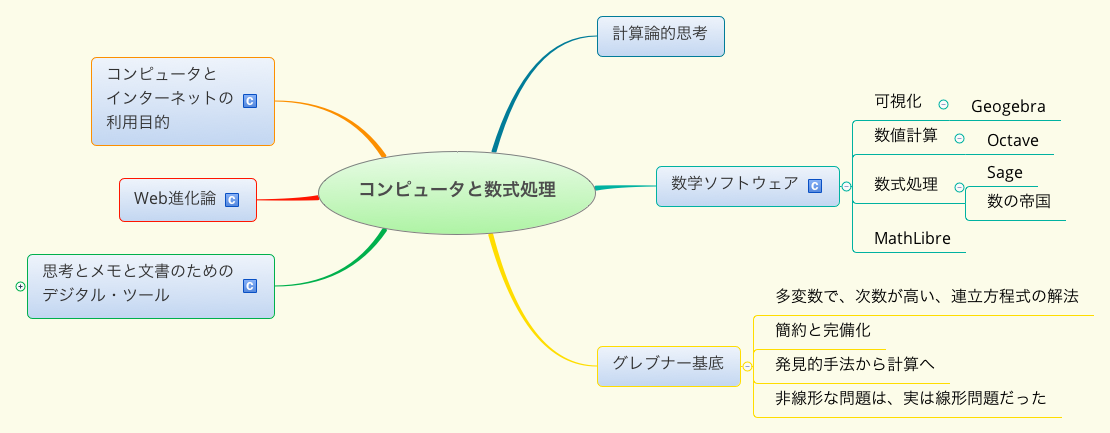
\includegraphics[width=.9\linewidth]{./map-images/01-computer_and_cal.png}
\end{center}

\section{過去の研究内容と興味}
\label{sec:orgf3da361}
\begin{center}
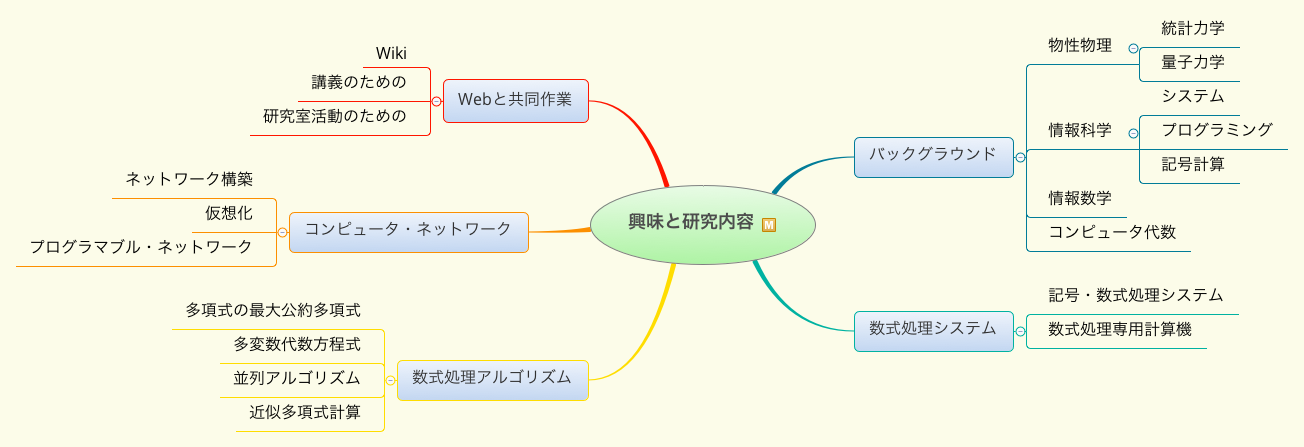
\includegraphics[width=.9\linewidth]{./map-images/02-research_interests.png}
\end{center}

\section{計算論的思考 (別紙)}
\label{sec:org09cca8b}

コンピュータ科学に基く概念とアプローチ法

\begin{itemize}
\item \url{./computationa\_thinking.org}
\end{itemize}


\section{デジタル・ツールとインターネット}
\label{sec:orgb8d1f2e}

\subsection{インターネットが起している変革}
\label{sec:org3c1e60f}
\begin{center}
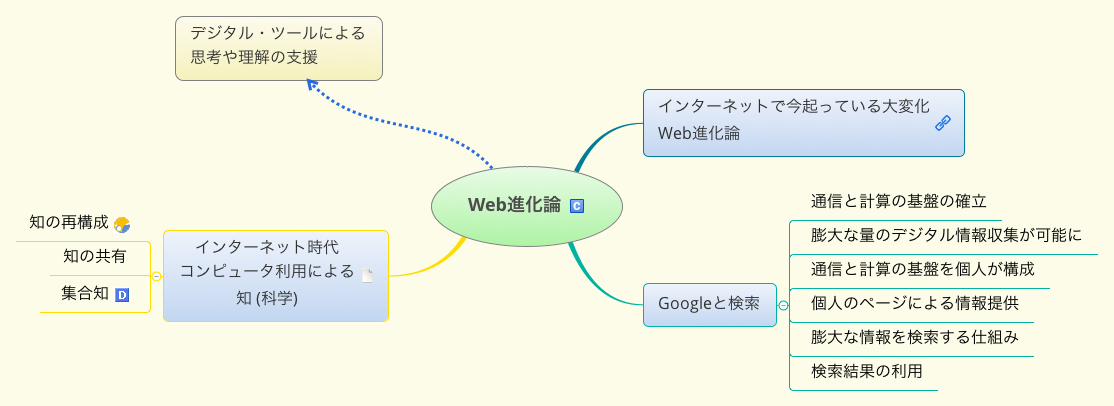
\includegraphics[width=.9\linewidth]{./map-images/04-Web_revolution.png}
\end{center}

\subsection{人間とコンピュータとインターネット}
\label{sec:org6336cc7}
\begin{center}
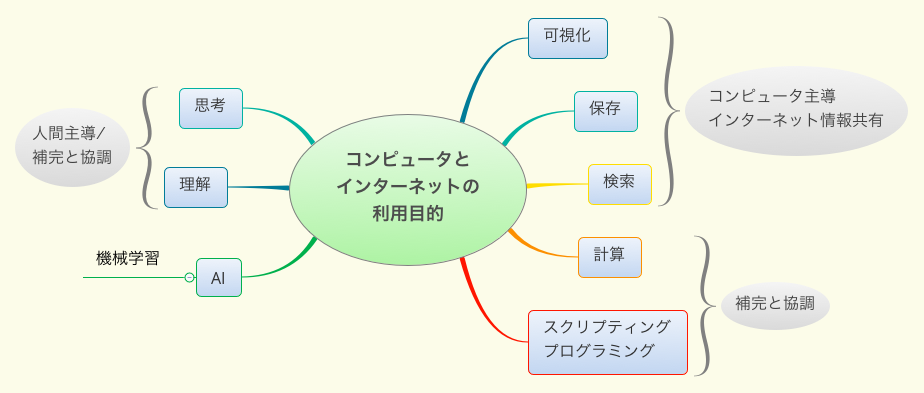
\includegraphics[width=.9\linewidth]{./map-images/03-how_to_use_computer_and_internet.png}
\end{center}

\subsection{思考とメモと文書のためのデジタル・ツール}
\label{sec:org3634110}
\begin{center}
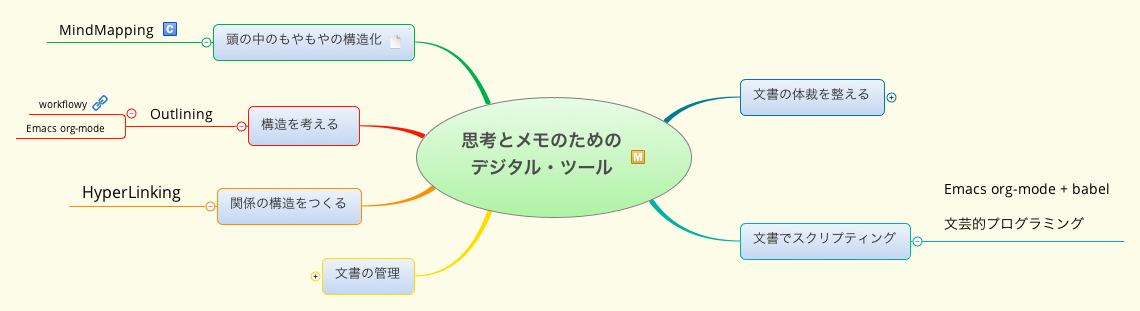
\includegraphics[width=.9\linewidth]{./map-images/05-digital_tools_for_thinking.png}
\end{center}

\section{数学ソフトウェア (別紙)}
\label{sec:orgc60b269}

\begin{itemize}
\item \url{./math-soft.org}
\end{itemize}

\subsection{数式処理システム Sage の紹介 (別紙)}
\label{sec:org79cfd0a}

\subsection{グレブナー基底とは (別紙)}
\label{sec:org5682027}

数式処理アルゴリズムの紹介


\begin{itemize}
\item \url{./gbasis.org}
\end{itemize}
\end{document}
